\chapter{Kristal I: Kristal Sempurna dan Logam}\label{ch:b1:crystals-metals}

Kawat tembaga dapat ditarik lebih tipis daripada rambut tanpa putus;
sebongkah garam hancur berkeping-keping di bawah pukulan palu. Seorang
pandai besi memanaskan sebatang besi sampai berpijar, menempanya,
mencelupkannya ke dalam air, dan batang itu keluar jauh lebih keras
daripada ketika masuk. Perbedaan perilaku ini terletak pada cara
atom-atom bertumpuk di dalam padatan. Kebanyakan padatan adalah \omterm{def:b1:crystals-metals:crystal}{kristal}:
atom-atomnya menempati sebuah pola yang berulang, identik, miliaran kali
ke segala arah. Bab ini memerikan pola-pola semacam itu, menghitung
atom-atomnya, mengukur seberapa rapat atom-atom itu tersusun dan di mana
celah-celah di antaranya berada, lalu memakai hasilnya untuk memahami
logam dan paduan. Bab berikutnya menerapkan alat-alat yang sama pada
padatan ion, kovalen, dan molekuler.

\begin{recall}
Logam mudah melepaskan \omterm{def:b1:quantum-numbers:configuration}{elektron valensinya}: energi ionisasi dan
\omterm{def:b1:periodicity:electronegativity}{keelektronegatifannya} rendah (\cref{ch:b1:periodicity}). Jari-jari atom
didefinisikan pada \cref{def:b1:periodicity:radius}. Massa jenis, sifat
yang dipelajari dalam fisika, dipakai sebagai hal yang sudah diketahui:
$\rho = m/V$.
\end{recall}

\begin{omfigure}
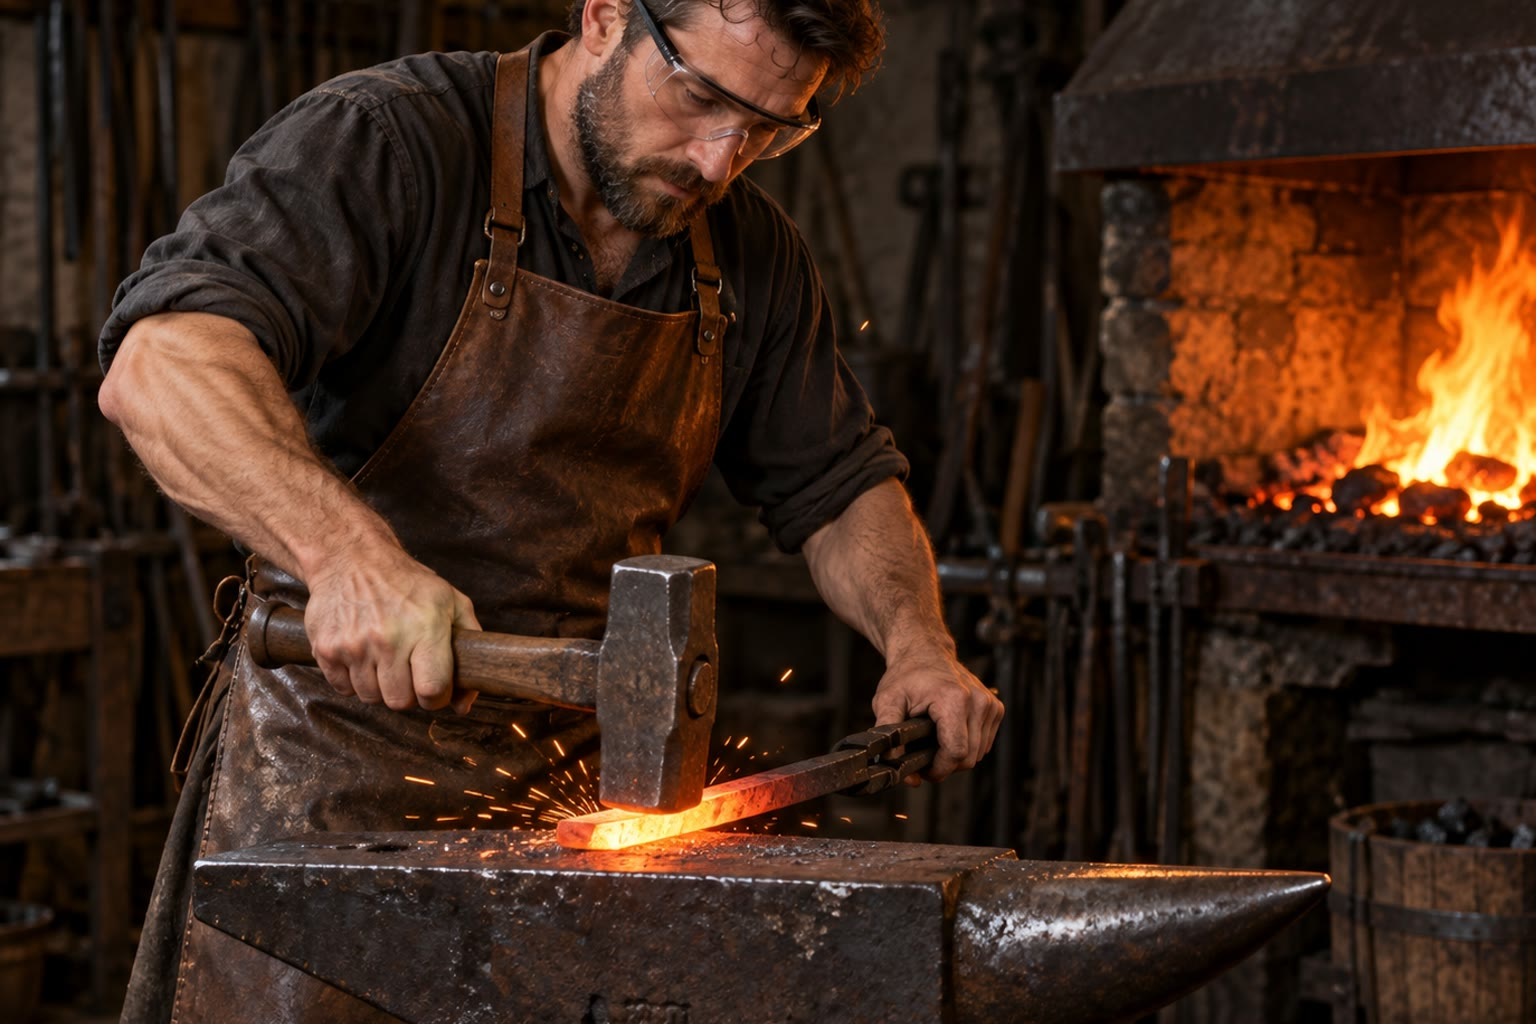
\includegraphics[width=0.55\linewidth]{images/book2/ai/b1-05-blacksmith.jpg}

{\small Seorang pandai besi menempa baja. Besi yang berpijar jingga
mempunyai struktur \omterm{def:b1:crystals-metals:crystal}{kristal} yang berbeda dari besi pada suhu kamar, dan
dapat menampung lebih banyak karbon (soal akhir pekan).}
\end{omfigure}

\section{Model kristal sempurna}

\begin{definition}[Kristal, padatan amorf, kristal sempurna]\label{def:b1:crystals-metals:crystal}
\emph{Kristal}\index{kristal} adalah padatan yang partikel-partikelnya
(atom, ion, atau molekul) tersusun dalam sebuah pola yang berulang
secara periodik dalam tiga dimensi. Padatan tanpa keteraturan jarak jauh
semacam itu adalah \emph{padatan amorf}\index{padatan amorf} (kaca,
kebanyakan plastik).
\emph{Model kristal sempurna}\index{model kristal sempurna} memerikan kristal sebagai benda yang tak berhingga dan tanpa
cacat: tanpa atom yang hilang atau berlebih, tanpa pengotor, tanpa
batas.
\end{definition}

\begin{definition}[Kisi, motif, sel satuan]\label{def:b1:crystals-metals:lattice}
\emph{Kisi}\index{kisi} adalah himpunan tak berhingga titik-titik, yaitu
\emph{simpul}\index{simpul}, yang diperoleh dari salah satunya melalui
semua translasi $u\,\vec a + v\,\vec b + w\,\vec c$ dengan $u$, $v$,
$w$ bilangan bulat. \omterm{def:b1:crystals-metals:crystal}{Kristal} diperoleh dengan menempatkan pada setiap
simpul \emph{motif}\index{motif} yang sama (satu atom, sekelompok atom
atau ion). \emph{Sel satuan}\index{sel satuan} adalah paralelepipedum
yang dibangun pada $\vec a$, $\vec b$, $\vec c$, yang translasi-translasinya
mengisi ruang; panjang rusuk dan sudut-sudutnya adalah \emph{parameter
kisi}\index{parameter kisi} $a$, $b$, $c$, $\alpha$, $\beta$, $\gamma$.
Pada sel kubus $a = b = c$ dan sudut-sudutnya $90^\circ$.
\end{definition}

\begin{remark}[Kristal nyata]\label{rem:b1:crystals-metals:real}
\omterm{def:b1:crystals-metals:crystal}{Kristal} nyata berhingga dan tidak sempurna: \omterm{def:b1:crystals-metals:crystal}{kristal} itu mengandung
kekosongan, pengotor, dislokasi, dan batas butir, yang mengendalikan
banyak sifat (keuletan tembaga, kekerasan baja). Cacat-cacat ini
dipelajari dalam jilid Tahun 3; \omterm{def:b1:crystals-metals:crystal}{kristal} sempurna memberikan geometri,
massa jenis, dan \omterm{def:b1:crystals-metals:compactness}{kekompakan}, yang hampir tidak diubah oleh cacat.
\end{remark}

\begin{definition}[Multiplisitas sebuah sel]\label{def:b1:crystals-metals:multiplicity}
\emph{Multiplisitas}\index{multiplisitas} $Z$ sebuah sel adalah banyaknya
\omterm{def:b1:crystals-metals:lattice}{motif} (atau atom) yang menjadi miliknya, dengan setiap atom yang dipakai
bersama sel-sel tetangga dihitung sebesar bagian yang terletak di dalam
sel itu.
\end{definition}

\begin{method}[Menghitung atom sebuah sel]\label{met:b1:crystals-metals:count}
Pada sel kubus, atom di sudut dipakai bersama oleh 8 sel dan dihitung
$1/8$; di rusuk dipakai bersama oleh 4 dan dihitung $1/4$; di muka
dipakai bersama oleh 2 dan dihitung $1/2$; di dalam dihitung 1.
Jumlahkan semua sumbangannya.
\end{method}

\begin{definition}[Bilangan koordinasi]\label{def:b1:crystals-metals:coordination}
\emph{Bilangan koordinasi}\index{bilangan koordinasi} sebuah partikel di
dalam padatan adalah banyaknya tetangga terdekatnya, yaitu yang berada
pada jarak terpendek.
\end{definition}

\begin{definition}[Kekompakan]\label{def:b1:crystals-metals:compactness}
\emph{Kekompakan}\index{kekompakan} (atau fraksi kemasan) sebuah \omterm{def:b1:crystals-metals:crystal}{kristal}
bola-bola keras adalah bagian volume yang ditempati bola-bola itu: untuk
sel bervolume $V$ yang memuat $Z$ bola berjari-jari $R$,
\[
  C = \frac{Z \cdot \frac43 \pi R^3}{V} .
\]
\end{definition}

\begin{proposition}[Massa jenis dari sel]\label{prop:b1:crystals-metals:density}
Massa jenis sebuah \omterm{def:b1:crystals-metals:crystal}{kristal} yang selnya, bervolume $V$, memuat $Z$
partikel bermassa molar $M$ adalah
\[
  \rho = \frac{Z\,M}{N_A\,V} .
\]
\end{proposition}

\begin{proof}
Sel itu memuat $Z$ partikel, yang massanya $Z\,M/N_A$; \omterm{def:b1:crystals-metals:crystal}{kristal} adalah
sel yang diulang-ulang, sehingga massa jenisnya sama dengan massa jenis
satu sel.
\end{proof}

\section{Susunan rapat: kubus berpusat muka dan heksagonal}

\begin{definition}[Susunan rapat, FCC, HCP]\label{def:b1:crystals-metals:packings}
\emph{Susunan rapat}\index{susunan rapat} bola-bola identik dibangun dari
lapisan-lapisan rapat, yang setiap bolanya menyentuh enam bola lain, dan
yang ditumpuk sedemikian sehingga setiap bola sebuah lapisan duduk di
sebuah cekungan lapisan di bawahnya. Tumpukan $ABCABC\dots$ menghasilkan
struktur \emph{kubus berpusat muka}\index{kubus berpusat muka} (FCC, atau
kubus rapat); tumpukan $ABAB\dots$ menghasilkan struktur
\emph{heksagonal rapat}\index{heksagonal rapat} (HCP). Struktur logam
ketiga, yang tidak rapat, adalah struktur \emph{kubus berpusat
badan}\index{kubus berpusat badan} (BCC), sebuah kubus dengan satu atom
di setiap sudut dan satu di pusatnya.
\end{definition}

\begin{omfigure}
\begin{tikzpicture}[font=\small]
  % layer A
  \foreach \i in {0,...,4} \foreach \j in {0,...,3} {
    \pgfmathsetmacro\x{\i+0.5*\j}
    \pgfmathsetmacro\y{0.866*\j}
    \draw[black!60, fill=omDef!25] (\x,\y) circle (0.5);
  }
  % layer B, in the hollows pointing up
  \foreach \i/\j in {1/0, 2/0, 3/0, 1/1, 2/1, 3/1, 1/2, 2/2} {
    \pgfmathsetmacro\x{\i+0.5*\j}
    \pgfmathsetmacro\y{0.866*\j+0.577}
    \draw[omThm!80!black, fill=omThm!25, fill opacity=0.75] (\x,\y) circle (0.5);
  }
  % C positions
  \foreach \i/\j in {1/0, 2/0, 3/0, 1/1, 2/1, 3/1} {
    \pgfmathsetmacro\x{\i+0.5+0.5*\j}
    \pgfmathsetmacro\y{0.866*\j+0.289}
    \fill[omMeth] (\x,\y) circle (0.11);
  }
  \node[anchor=west, align=left] at (6.6,1.6) {A: lapisan pertama (biru)\\B: lapisan kedua, di\\\phantom{B: }cekungan A (merah)\\C: cekungan lainnya\\\phantom{C: }(titik hijau)};
\end{tikzpicture}

{\small Dua lapisan rapat yang dilihat dari atas. Lapisan ketiga dapat
duduk di atas cekungan bertanda C (tumpukan $ABC$, \omterm{def:b1:crystals-metals:packings}{kubus berpusat muka})
atau di atas atom-atom A (tumpukan $AB$, \omterm{def:b1:crystals-metals:packings}{heksagonal rapat}).}
\end{omfigure}

\begin{proposition}[Kubus berpusat muka]\label{prop:b1:crystals-metals:fcc}
Pada struktur FCC, atom-atom menempati kedelapan sudut dan keenam pusat
muka sebuah kubus berusuk $a$. Maka $Z = 4$, \omterm{def:b1:crystals-metals:coordination}{bilangan koordinasinya} 12,
atom-atom bersentuhan sepanjang diagonal muka, $a\sqrt2 = 4R$, dan
\omterm{def:b1:crystals-metals:compactness}{kekompakannya}
\[
  C = \frac{\pi}{3\sqrt2} \approx 0.74 .
\]
\end{proposition}

\begin{proof}
$Z = 8 \times \frac18 + 6 \times \frac12 = 4$. Sebuah atom di pusat muka
menyentuh keempat sudut mukanya dan empat pusat muka pada masing-masing
kedua sel yang berbagi muka itu: $4 + 4 + 4 = 12$ tetangga pada jarak
$a\sqrt2/2$. Pada diagonal muka, yang panjangnya $a\sqrt2$, terletak
sebuah atom sudut, sebuah atom pusat muka, dan sebuah atom sudut yang
saling bersentuhan: $a\sqrt2 = 4R$. Maka
$C = 4 \cdot \frac43\pi R^3/a^3 = \frac{16}{3}\pi R^3/(2\sqrt2 R)^3 \cdot
\frac{1}{1} = \frac{16\pi}{3 \times 16\sqrt2} = \frac{\pi}{3\sqrt2}$.
\end{proof}

\begin{omfigure}
\tdplotsetmaincoords{60}{100}
\begin{tikzpicture}[tdplot_main_coords, font=\small]
  \pic {omcubeo={3}};
  \node[cellA=6mm] at (0,0,0) {};
  \node[cellA=6mm] at (0,3,0) {};
  \node[cellA=6mm, ball color=omDef!55] at (0,1.5,1.5) {};
  \node[cellA=6mm] at (0,0,3) {};
  \node[cellA=6mm, ball color=omDef!55] at (1.5,1.5,0) {};
  \node[cellA=6mm] at (0,3,3) {};
  \node[cellA=6mm, ball color=omDef!55] at (1.5,0,1.5) {};
  \node[cellA=6mm, ball color=omDef!55] at (1.5,3,1.5) {};
  \node[cellA=6mm] at (3,0,0) {};
  \node[cellA=6mm, ball color=omDef!55] at (1.5,1.5,3) {};
  \node[cellA=6mm] at (3,3,0) {};
  \node[cellA=6mm, ball color=omDef!55] at (3,1.5,1.5) {};
  \node[cellA=6mm] at (3,0,3) {};
  \node[cellA=6mm] at (3,3,3) {};
  \draw[omThm, thick] (3,0,0) -- (3,3,3);
\end{tikzpicture}
\hspace{1.2cm}
\begin{tikzpicture}[tdplot_main_coords, font=\small]
  \pic {omcubeo={3}};
  \node[cellA=7mm] at (0,0,0) {};
  \node[cellA=7mm] at (0,3,0) {};
  \node[cellA=7mm] at (0,0,3) {};
  \node[cellA=7mm] at (0,3,3) {};
  \node[cellA=7mm, ball color=omDef!55] at (1.5,1.5,1.5) {};
  \node[cellA=7mm] at (3,0,0) {};
  \node[cellA=7mm] at (3,3,0) {};
  \node[cellA=7mm] at (3,0,3) {};
  \node[cellA=7mm] at (3,3,3) {};
  \draw[omThm, thick] (3,0,0) -- (0,3,3);
\end{tikzpicture}

{\small Kiri: sel \omterm{def:b1:crystals-metals:packings}{kubus berpusat muka} (atom sudut abu-abu, atom pusat
muka biru). Atom-atom bersentuhan sepanjang diagonal muka (garis merah,
$a\sqrt2 = 4R$). Kanan: sel \omterm{def:b1:crystals-metals:packings}{kubus berpusat badan}; atom-atom bersentuhan
sepanjang diagonal ruang (garis merah, $a\sqrt3 = 4R$). Atom-atom
digambar lebih kecil daripada ukuran sentuhnya, agar jelas.}
\end{omfigure}

\begin{proposition}[Heksagonal rapat]\label{prop:b1:crystals-metals:hcp}
Pada struktur HCP, prisma heksagonal konvensional, dengan rusuk alas $a$
dan tinggi $c$, memuat 6 atom; \omterm{def:b1:crystals-metals:coordination}{bilangan koordinasinya} 12; untuk bola-bola
yang bersentuhan $a = 2R$, $c/a = \sqrt{8/3} \approx 1.633$, dan
\omterm{def:b1:crystals-metals:compactness}{kekompakannya} sama dengan \omterm{def:b1:crystals-metals:compactness}{kekompakan} FCC, $\pi/(3\sqrt2) \approx 0.74$.
\end{proposition}

\begin{proof}
Prisma itu mempunyai 12 atom sudut yang dipakai bersama oleh 6 prisma,
2 atom pusat muka yang dipakai bersama oleh 2, dan 3 atom di dalamnya:
$12/6 + 2/2 + 3 = 6$. Setiap atom menyentuh enam tetangga dalam
lapisannya dan tiga pada setiap lapisan yang berdampingan: 12. Sebuah atom
lapisan B duduk di atas tiga atom lapisan A yang saling bersentuhan,
membentuk tetrahedron beraturan berusuk $2R$, yang tingginya
$2R\sqrt{2/3}$; dua lapisan berjarak $c = 4R\sqrt{2/3}$, sehingga
$c/a = 2\sqrt{2/3} = \sqrt{8/3}$. Volume prisma adalah
$\frac{3\sqrt3}{2}a^2 c = \frac{3\sqrt3}{2}(2R)^2 \cdot
4R\sqrt{2/3} = 24\sqrt2\,R^3$, dan $C = 6 \cdot \frac43\pi R^3/(24\sqrt2
R^3) = \pi/(3\sqrt2)$.
\end{proof}

\begin{omfigure}
\tdplotsetmaincoords{70}{113}
\begin{tikzpicture}[tdplot_main_coords, font=\small, scale=1.25]
  \pic[transform shape] {omhexprismo={1.6}{2.6}};
  \node[cellA=6mm] at (-1.6,0,0) {};
  \node[cellA=6mm] at (-0.8,-1.386,0) {};
  \node[cellA=6mm] at (-1.6,0,2.6) {};
  \node[cellA=6mm] at (-0.8,-1.386,2.6) {};
  \node[cellA=6mm] at (-0.8,1.386,0) {};
  \node[cellA=6mm, ball color=omThm!60] at (-0.8,0.462,1.3) {};
  \node[cellA=6mm] at (0,0,0) {};
  \node[cellA=6mm, ball color=omThm!60] at (0,-0.924,1.3) {};
  \node[cellA=6mm] at (0.8,-1.386,0) {};
  \node[cellA=6mm] at (-0.8,1.386,2.6) {};
  \node[cellA=6mm] at (0,0,2.6) {};
  \node[cellA=6mm] at (0.8,-1.386,2.6) {};
  \node[cellA=6mm] at (0.8,1.386,0) {};
  \node[cellA=6mm, ball color=omThm!60] at (0.8,0.462,1.3) {};
  \node[cellA=6mm] at (1.6,0,0) {};
  \node[cellA=6mm] at (0.8,1.386,2.6) {};
  \node[cellA=6mm] at (1.6,0,2.6) {};
\end{tikzpicture}

{\small Prisma \omterm{def:b1:crystals-metals:packings}{heksagonal rapat}, dengan rusuk alas $a$ (sisi segi enam)
dan tinggi $c$: lapisan A (abu-abu) di bawah dan di atas, lapisan B
(merah) di tengah, duduk di cekungan-cekungan A.}
\end{omfigure}

\section{Kubus berpusat badan dan unsur-unsur logam}

\begin{proposition}[Kubus berpusat badan]\label{prop:b1:crystals-metals:bcc}
Pada struktur BCC $Z = 2$, \omterm{def:b1:crystals-metals:coordination}{bilangan koordinasinya} 8, atom-atom
bersentuhan sepanjang diagonal ruang kubus, $a\sqrt3 = 4R$, dan
\omterm{def:b1:crystals-metals:compactness}{kekompakannya}
\[
  C = \frac{\pi\sqrt3}{8} \approx 0.68 .
\]
\end{proposition}

\begin{proof}
$Z = 8 \times \frac18 + 1 = 2$. Atom pusat menyentuh kedelapan sudut:
diagonal ruang $a\sqrt3$ memuat sebuah atom sudut, atom pusat, dan
sebuah atom sudut, $a\sqrt3 = 4R$. Maka $C = 2 \cdot \frac43\pi R^3/a^3 =
\frac83\pi R^3 (\sqrt3/(4R))^3 = \frac83\pi \cdot \frac{3\sqrt3}{64} =
\frac{\pi\sqrt3}{8}$.
\end{proof}

\begin{proposition}[Susunan rapat adalah yang terpadat]\label{prop:b1:crystals-metals:kepler}
Tidak ada susunan bola-bola identik yang \omterm{def:b1:crystals-metals:compactness}{kekompakannya} lebih besar
daripada $\pi/(3\sqrt2) \approx 0.7405$, nilai untuk FCC dan HCP.
\end{proposition}
\admitted

\begin{history}[Konjektur Kepler, 1611--2017]
Dalam sebuah esai pendek tentang kepingan salju, yang ditulis pada tahun
1611, Johannes Kepler menyatakan bahwa tidak ada cara menumpuk peluru
meriam yang lebih padat daripada piramida pedagang buah, yaitu susunan
\omterm{def:b1:crystals-metals:packings}{kubus berpusat muka}. Pernyataan itu menolak dibuktikan selama hampir
empat abad. Thomas Hales memberikan bukti berbantuan komputer pada tahun
1998, dan sebuah bukti formal yang diperiksa baris demi baris oleh
komputer diselesaikan pada tahun 2014 dan diterbitkan pada tahun 2017.
\end{history}

\begin{example}[Tiga logam]\label{ex:b1:crystals-metals:metals}
Tembaga berstruktur FCC dengan $a = \qty{361.5}{pm}$: $R = a\sqrt2/4 =
\qty{127.8}{pm}$ dan $\rho = 4 \times 63.55/(6.022 \times 10^{23} \times
(3.615 \times 10^{-8})^3) = \qty{8.93}{g/cm^3}$, massa jenis terukurnya.
Besi pada suhu kamar (besi-$\alpha$) berstruktur BCC dengan
$a = \qty{286.7}{pm}$: $R = \qty{124.1}{pm}$, $\rho = \qty{7.87}{g/cm^3}$.
Magnesium berstruktur HCP dengan $a = \qty{320.9}{pm}$ dan
$c = \qty{521.0}{pm}$: $c/a = 1.624$, mendekati nilai ideal $1.633$;
seng, dengan $c/a = 1.856$, adalah susunan heksagonal yang memanjang.
% ledger: lat:Cu, rho:Cu, lat:Fe-alpha, rho:Fe, lat:Mg.a, lat:Mg.c,
% lat:Zn.a, lat:Zn.c, aw:Cu, aw:Fe, const:NA
\end{example}

\begin{center}
\small
\begin{tabular}{lllccc}
\hline
logam & struktur & $a$ (pm) & $R$ (pm) & $\rho$ terhitung & $\rho$ terukur \\
\hline
aluminium & FCC & 405.0 & 143.2 & 2.70 & 2.70 \\
tembaga & FCC & 361.5 & 127.8 & 8.93 & 8.93 \\
perak & FCC & 408.6 & 144.5 & 10.50 & 10.50 \\
natrium & BCC & 429.1 & 185.8 & 0.967 & 0.97 \\
besi-$\alpha$ & BCC & 286.7 & 124.1 & 7.87 & 7.87 \\
wolfram & BCC & 316.5 & 137.0 & 19.26 & 19.3 \\
\hline
\end{tabular}
\end{center}
% ledger: lat:Al, lat:Cu, lat:Ag, lat:Na, lat:Fe-alpha, lat:W, rho:Al,
% rho:Cu, rho:Ag, rho:Na, rho:Fe, rho:W (densities in g/cm3)

\begin{omfigure}
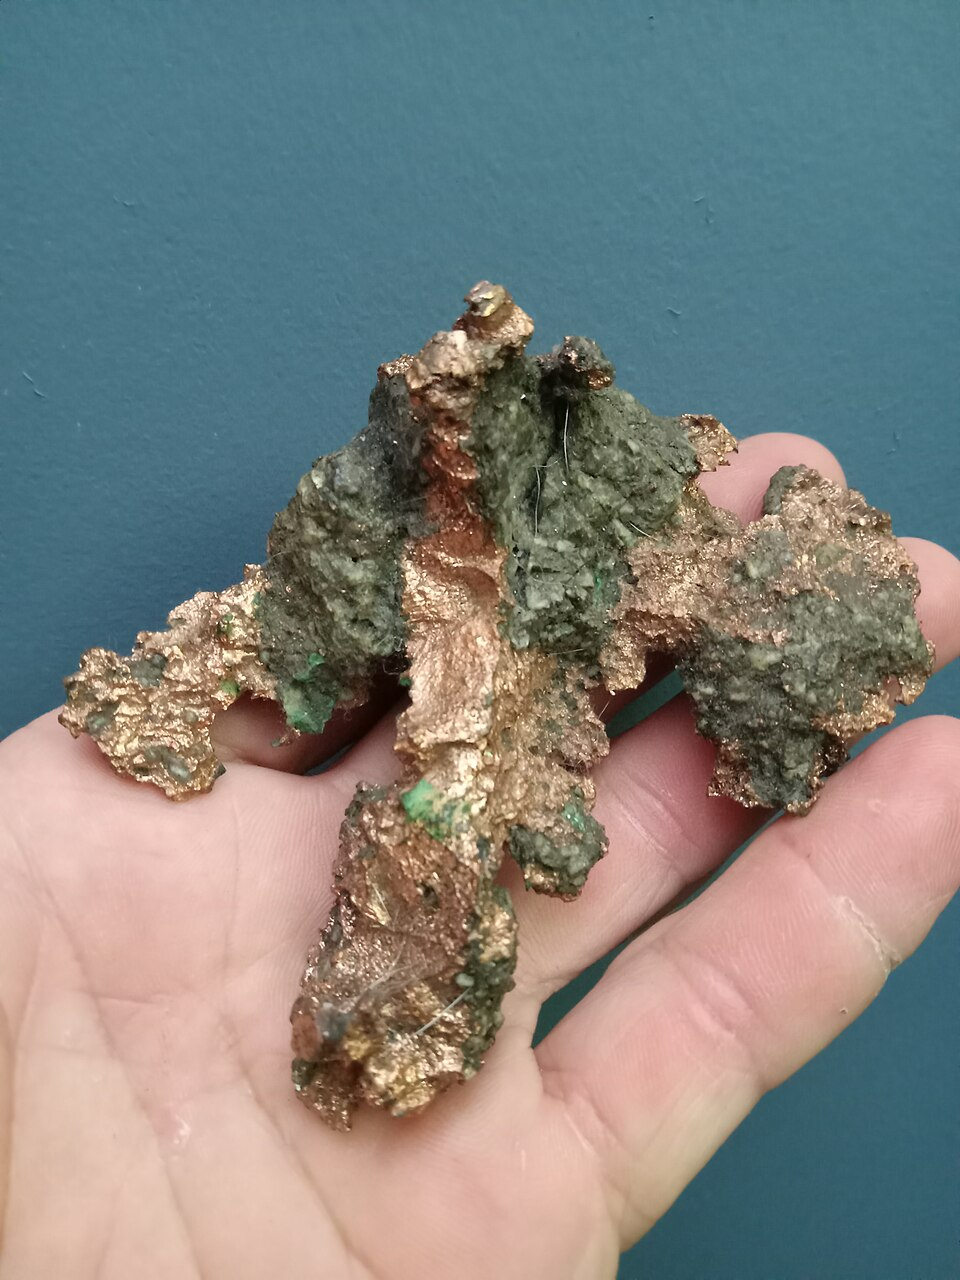
\includegraphics[width=0.36\linewidth]{images/book2/native-copper.jpg}

{\small Spesimen tembaga murni alami. Bentuk-bentuknya yang bercabang
tumbuh sebagai \omterm{def:b1:crystals-metals:crystal}{kristal}; logam di bawahnya adalah mozaik butir-butir FCC.
Foto: CC0 (Wikimedia Commons).}
\end{omfigure}

\section{Situs interstisi}

\begin{definition}[Situs interstisi]\label{def:b1:crystals-metals:site}
\emph{Situs interstisi}\index{situs interstisi} adalah celah di antara
atom-atom sebuah \omterm{def:b1:crystals-metals:crystal}{kristal} yang dapat ditempati atom yang lebih kecil.
\emph{Situs tetrahedral}\index{situs tetrahedral} terletak di pusat
tetrahedron yang dibentuk empat atom,
\emph{situs oktahedral}\index{situs oktahedral} di pusat oktahedron yang dibentuk enam atom.
\emph{Keterhunian}\index{keterhunian} sebuah situs adalah jari-jari bola
terbesar yang muat di dalamnya tanpa mendorong atom-atom di sekitarnya
menjauh.
\end{definition}

\begin{proposition}[Situs-situs struktur FCC]\label{prop:b1:crystals-metals:sites}
Sebuah sel FCC memuat 4 \omterm{def:b1:crystals-metals:site}{situs oktahedral}, di pusat kubus dan di titik
tengah ke-12 rusuknya, serta 8 \omterm{def:b1:crystals-metals:site}{situs tetrahedral}, di pusat kedelapan
kubus kecil berusuk $a/2$. Untuk atom-atom berjari-jari $R$ yang
bersentuhan, \omterm{def:b1:crystals-metals:site}{keterhuniannya} adalah
\[
  r_O = (\sqrt2 - 1)R \approx 0.414\,R, \qquad
  r_T = \left(\sqrt{\tfrac32} - 1\right)R \approx 0.225\,R .
\]
\end{proposition}

\begin{proof}
\omterm{def:b1:crystals-metals:site}{Situs oktahedral}: $1 + 12 \times \frac14 = 4$, sama banyak dengan
atomnya. Pusat kubus berjarak $a/2$ dari keenam pusat muka:
$r_O + R = a/2$ dengan $a = 2\sqrt2 R$, sehingga $r_O = (\sqrt2 - 1)R$.
\omterm{def:b1:crystals-metals:site}{Situs tetrahedral}: pusat kubus kecil berusuk $a/2$ berjarak setengah
diagonal ruangnya, $\frac{a}{2}\cdot\frac{\sqrt3}{2} = \frac{a\sqrt3}{4}$,
dari keempat atom di sudut-sudut yang berselang-seling:
$r_T + R = \frac{\sqrt3}{4}\,2\sqrt2\,R =
\sqrt{\tfrac32}\,R$.
\end{proof}

\begin{omfigure}
\tdplotsetmaincoords{60}{100}
\begin{tikzpicture}[tdplot_main_coords, font=\small]
  \pic {omcubeo={3}};
  \node[cellA=3.6mm] at (0,0,0) {};
  \node[cellsite=4mm, draw=omThm, fill=omThm!30] at (0,1.5,0) {};
  \node[cellA=3.6mm] at (0,3,0) {};
  \node[cellsite=4mm, draw=omThm, fill=omThm!30] at (0,0,1.5) {};
  \node[cellA=3.6mm] at (0,1.5,1.5) {};
  \node[cellsite=4mm, draw=omThm, fill=omThm!30] at (0,3,1.5) {};
  \node[cellsite=4mm, draw=omThm, fill=omThm!30] at (1.5,0,0) {};
  \node[cellA=3.6mm] at (0,0,3) {};
  \node[cellA=3.6mm] at (1.5,1.5,0) {};
  \node[cellsite=4mm, draw=omThm, fill=omThm!30] at (0,1.5,3) {};
  \node[cellsite=4mm, draw=omThm, fill=omThm!30] at (1.5,3,0) {};
  \node[cellA=3.6mm] at (0,3,3) {};
  \node[cellA=3.6mm] at (1.5,0,1.5) {};
  \node[cellsite=5mm, draw=omThm, fill=omThm!30] at (1.5,1.5,1.5) {};
  \node[cellA=3.6mm] at (1.5,3,1.5) {};
  \node[cellA=3.6mm] at (3,0,0) {};
  \node[cellsite=4mm, draw=omThm, fill=omThm!30] at (1.5,0,3) {};
  \node[cellsite=4mm, draw=omThm, fill=omThm!30] at (3,1.5,0) {};
  \node[cellA=3.6mm] at (1.5,1.5,3) {};
  \node[cellA=3.6mm] at (3,3,0) {};
  \node[cellsite=4mm, draw=omThm, fill=omThm!30] at (1.5,3,3) {};
  \node[cellsite=4mm, draw=omThm, fill=omThm!30] at (3,0,1.5) {};
  \node[cellA=3.6mm] at (3,1.5,1.5) {};
  \node[cellsite=4mm, draw=omThm, fill=omThm!30] at (3,3,1.5) {};
  \node[cellA=3.6mm] at (3,0,3) {};
  \node[cellsite=4mm, draw=omThm, fill=omThm!30] at (3,1.5,3) {};
  \node[cellA=3.6mm] at (3,3,3) {};
  \node[below] at (1.5,1.5,-1.5) {situs oktahedral (merah)};
\end{tikzpicture}
\hspace{1.2cm}
\begin{tikzpicture}[tdplot_main_coords, font=\small]
  \pic {omcubeo={3}};
  \node[cellA=3.6mm] at (0,0,0) {};
  \node[cellA=3.6mm] at (0,3,0) {};
  \node[cellA=3.6mm] at (0,1.5,1.5) {};
  \node[cellsite=4mm, fill=omDef!30] at (0.75,0.75,0.75) {};
  \node[cellsite=4mm, fill=omDef!30] at (0.75,2.25,0.75) {};
  \node[cellA=3.6mm] at (0,0,3) {};
  \node[cellA=3.6mm] at (1.5,1.5,0) {};
  \node[cellsite=4mm, fill=omDef!30] at (0.75,0.75,2.25) {};
  \node[cellA=3.6mm] at (0,3,3) {};
  \node[cellA=3.6mm] at (1.5,0,1.5) {};
  \node[cellsite=4mm, fill=omDef!30] at (0.75,2.25,2.25) {};
  \node[cellsite=4mm, fill=omDef!30] at (2.25,0.75,0.75) {};
  \node[cellA=3.6mm] at (1.5,3,1.5) {};
  \node[cellA=3.6mm] at (3,0,0) {};
  \node[cellsite=4mm, fill=omDef!30] at (2.25,2.25,0.75) {};
  \node[cellA=3.6mm] at (1.5,1.5,3) {};
  \node[cellA=3.6mm] at (3,3,0) {};
  \node[cellsite=4mm, fill=omDef!30] at (2.25,0.75,2.25) {};
  \node[cellsite=4mm, fill=omDef!30] at (2.25,2.25,2.25) {};
  \node[cellA=3.6mm] at (3,1.5,1.5) {};
  \node[cellA=3.6mm] at (3,0,3) {};
  \node[cellA=3.6mm] at (3,3,3) {};
  \draw[omDef!70!black, thin] (0,0,0) -- (0.75,0.75,0.75) -- (1.5,1.5,0)
    (0.75,0.75,0.75) -- (1.5,0,1.5) (0.75,0.75,0.75) -- (0,1.5,1.5);
  \node[below] at (1.5,1.5,-1.5) {situs tetrahedral (biru)};
\end{tikzpicture}

{\small Situs-situs interstisi sel FCC. Kiri: \omterm{def:b1:crystals-metals:site}{situs oktahedral} di pusat
dan situs-situs di titik tengah rusuk (dipakai bersama oleh empat sel).
Kanan: kedelapan \omterm{def:b1:crystals-metals:site}{situs tetrahedral} di pusat seperdelapan-seperdelapan
kubus, salah satunya digambar terhubung dengan keempat atomnya.}
\end{omfigure}

\section{Ikatan logam dan paduan}

\begin{definition}[Ikatan logam]\label{def:b1:crystals-metals:metallic-bond}
Dalam \emph{ikatan logam}\index{ikatan logam}, setiap atom logam
menyerahkan \omterm{def:b1:quantum-numbers:configuration}{elektron valensinya} kepada seluruh \omterm{def:b1:crystals-metals:crystal}{kristal}: padatan itu
adalah \omterm{def:b1:crystals-metals:lattice}{kisi} kation yang bermandikan elektron-elektron yang bukan milik
atom tertentu mana pun dan bergerak bebas di dalamnya. Ikatan ini adalah
tarikan antara kation-kation dan awan elektron bersama itu; ikatan ini
tidak terarah.
\end{definition}

\begin{proposition}[Sifat-sifat logam]\label{prop:b1:crystals-metals:properties}
\omterm{def:b1:crystals-metals:metallic-bond}{Ikatan logam} menjelaskan sifat-sifat logam: elektron-elektron yang
bergerak bebas menghantarkan listrik dan kalor serta memantulkan cahaya
(kilap); karena ikatannya tidak terarah, lapisan-lapisan atom dapat
bergeser satu terhadap yang lain tanpa memecahkan \omterm{def:b1:crystals-metals:crystal}{kristal} (keuletan,
kemudahan ditempa), dan \omterm{def:b1:crystals-metals:packings}{susunan rapat}, yang memaksimalkan banyaknya
tetangga, adalah struktur yang paling umum.
\end{proposition}
\admitted

\begin{definition}[Paduan]\label{def:b1:crystals-metals:alloy}
Paduan adalah padatan logam yang tersusun atas beberapa unsur. Dalam
\emph{paduan substitusi}\index{paduan substitusi}, atom-atom unsur yang
ditambahkan menggantikan atom-atom unsur induk pada \omterm{def:b1:crystals-metals:lattice}{kisinya}; hal ini
memerlukan jari-jari yang selisihnya tidak lebih dari sekitar 15\,\%
(tembaga dan nikel, tembaga dan seng dalam kuningan). Dalam
\emph{paduan interstisi}\index{paduan interstisi}, atom-atom kecil
(\ce{H}, \ce{C}, \ce{N}, \ce{B}) menempati situs-situs interstisi unsur
induk (karbon dalam baja).
\end{definition}

\begin{definition}[Alotropi]\label{def:b1:crystals-metals:allotropy}
Struktur-struktur \omterm{def:b1:crystals-metals:crystal}{kristal} yang berbeda dari unsur yang sama adalah
\emph{alotrop}\index{alotrop} unsur itu. Besi berstruktur BCC
(besi-$\alpha$) pada suhu kamar; struktur FCC (besi-$\gamma$) teramati
dari \qty{1189}{K} sampai \qty{1661}{K}, dan struktur BCC kembali
(besi-$\delta$) pada \qty{1662}{K}, sampai titik lelehnya. Karbon
terdapat sebagai intan dan sebagai grafit
(\cref{ch:b1:crystals-ionic-covalent}).
% ledger: lat:Fe-alpha, lat:Fe-gamma-1189, lat:Fe-gamma-1661,
% lat:Fe-delta-1662
\end{definition}

\begin{example}[Baja]\label{ex:b1:crystals-metals:steel}
Karbon, dengan \omterm{def:b1:periodicity:radius}{jari-jari kovalen} \qty{77}{pm} (setengah jarak \ce{C-C}
dalam intan), terlalu besar untuk situs-situs besi tanpa distorsi, tetapi
jauh lebih tidak demikian pada besi-$\gamma$, yang \omterm{def:b1:crystals-metals:site}{situs oktahedralnya}
paling besar. Baja dibuat dengan melarutkan karbon dalam besi-$\gamma$
yang panas; jika dicelup cepat, karbon terperangkap ketika besi kembali
ke struktur berpusat badan, yang didistorsinya, dan \omterm{def:b1:crystals-metals:crystal}{kristal} yang
terdistorsi itu keras.
% ledger: lat:C-diamond (r = a sqrt3 / 8 = 77.2 pm)
\end{example}

\begin{remark}[Transisi-transisi besi]\label{rem:b1:crystals-metals:iron-T}
Suhu-suhu pada \cref{def:b1:crystals-metals:allotropy} adalah suhu untuk
besi murni pada tekanan atmosfer; karbon yang terlarut menurunkan suhu
terbentuknya besi-$\gamma$, yang membuat baja dapat dikerjakan. Diagram
fase paduan dipelajari dalam jilid Tahun 2.
\end{remark}

\section{Latihan}

\begin{exercise}[$\star$]\label{exo:b1:crystals-metals:1}
Hitunglah atom-atom sel kubus sederhana (atom hanya di sudut-sudut), sel
BCC, dan sel FCC, lalu sebutkan \omterm{def:b1:crystals-metals:coordination}{bilangan koordinasi} masing-masing.
\end{exercise}

\begin{exercise}[$\star$]\label{exo:b1:crystals-metals:2}
Tunjukkan bahwa \omterm{def:b1:crystals-metals:compactness}{kekompakan} struktur kubus sederhana (atom-atom bersentuhan
sepanjang rusuk) adalah $\pi/6$, lalu bandingkan dengan FCC dan BCC.
\end{exercise}

\begin{exercise}[$\star$]\label{exo:b1:crystals-metals:3}
Aluminium berstruktur FCC dengan $a = \qty{405.0}{pm}$. Hitunglah
jari-jari atomnya dan massa jenisnya ($M = \qty{26.98}{g/mol}$).
% ledger: lat:Al, aw:Al
\end{exercise}

\begin{exercise}[$\star$]\label{exo:b1:crystals-metals:4}
Natrium berstruktur BCC dengan $a = \qty{429.1}{pm}$. Hitunglah jari-jari
atomnya dan massa jenisnya ($M = \qty{22.99}{g/mol}$), lalu bandingkan
dengan nilai terukur \qty{0.97}{g/cm^3}.
% ledger: lat:Na, rho:Na, aw:Na
\end{exercise}

\begin{exercise}[$\star\star$]\label{exo:b1:crystals-metals:5}
Perak berstruktur FCC dan massa jenisnya \qty{10.50}{g/cm^3}
($M = \qty{107.87}{g/mol}$). Hitunglah \omterm{def:b1:crystals-metals:lattice}{parameter kisi} dan jari-jari
atomnya.
% ledger: rho:Ag, aw:Ag
\end{exercise}

\begin{exercise}[$\star\star$]\label{exo:b1:crystals-metals:6}
Tunjukkan bahwa pada struktur HCP dengan bola-bola yang bersentuhan
$c/a = \sqrt{8/3}$. Magnesium mempunyai $a = \qty{320.9}{pm}$,
$c = \qty{521.0}{pm}$. Hitunglah $c/a$ dan massa jenis magnesium
($M = \qty{24.31}{g/mol}$).
% ledger: lat:Mg.a, lat:Mg.c, aw:Mg
\end{exercise}

\begin{exercise}[$\star\star$]\label{exo:b1:crystals-metals:7}
Dalam sel FCC berusuk $a$, tuliskan koordinat keempat atom yang menjadi
milik sel itu, keempat \omterm{def:b1:crystals-metals:site}{situs oktahedral}, dan kedelapan \omterm{def:b1:crystals-metals:site}{situs tetrahedral}.
Berapa banyak masing-masing per atom?
\end{exercise}

\begin{exercise}[$\star\star$]\label{exo:b1:crystals-metals:8}
Tembaga dan nikel sama-sama berstruktur FCC, dengan $a = \qty{361.5}{pm}$
dan $a = \qty{352.4}{pm}$. Hitunglah jari-jari atomnya. Keduanya membentuk
\omterm{def:b1:crystals-metals:alloy}{paduan substitusi} dalam segala perbandingan: jelaskan. Paduan jenis apa
yang dapat dibentuk hidrogen, atom yang sangat kecil, dengan sebuah logam?
% ledger: lat:Cu, lat:Ni
\end{exercise}

\begin{exercise}[$\star\star$]\label{exo:b1:crystals-metals:9}
Wolfram berstruktur BCC dengan $a = \qty{316.5}{pm}$. Hitunglah
jari-jarinya, massa jenisnya ($M = \qty{183.84}{g/mol}$), dan banyaknya
atom dalam \qty{1}{cm^3}.
% ledger: lat:W, aw:W
\end{exercise}

\begin{exercise}[$\star\star\star$]\label{exo:b1:crystals-metals:10}
Pada struktur BCC, sebuah \omterm{def:b1:crystals-metals:site}{situs oktahedral} terletak di pusat setiap muka
(dan di titik tengah setiap rusuk), dan sebuah \omterm{def:b1:crystals-metals:site}{situs tetrahedral} di
$(\frac{a}{2}, \frac{a}{4}, 0)$ pada setiap muka. Tunjukkan bahwa
\omterm{def:b1:crystals-metals:site}{keterhuniannya} adalah $r_O = \frac{2 - \sqrt3}{4}\,a$ dan
$r_T = \frac{\sqrt5 - \sqrt3}{4}\,a$, lalu nyatakan keduanya sebagai
bagian dari $R$. Situs manakah yang lebih besar?
\end{exercise}

\begin{exercise}[$\star\star\star$]\label{exo:b1:crystals-metals:11}
Sebuah logam mengkristal dengan $Z$ atom per sel kubus berusuk $a$.
Tunjukkan bahwa \omterm{def:b1:crystals-metals:compactness}{kekompakannya} dapat ditulis $C = \frac{4\pi R^3 Z}{3a^3}$,
lalu bahwa $C = \frac{\pi\rho N_A}{6M}\,(2R)^3$. Terapkan pada tembaga
($R = \qty{127.8}{pm}$, $\rho = \qty{8.93}{g/cm^3}$) untuk memeriksa
nilai $0.74$.
\end{exercise}

\begin{exercise}[$\star\star\star$]\label{exo:b1:crystals-metals:12}
Emas berstruktur FCC dengan $a = \qty{407.8}{pm}$ dan perak FCC dengan
$a = \qty{408.6}{pm}$. Emas dan perak bercampur dalam segala perbandingan.
Perkirakan \omterm{def:b1:crystals-metals:lattice}{parameter kisi} paduan yang mengandung 50\,\% atom
masing-masing (anggaplah sama dengan rata-ratanya) dan massa jenisnya
($M(\ce{Au}) = \qty{196.97}{g/mol}$, $M(\ce{Ag}) = \qty{107.87}{g/mol}$).
% ledger: lat:Au, lat:Ag, aw:Au, aw:Ag
\end{exercise}

\section{Soal: Mengapa Baja Menampung Karbon}

\begin{problem}[{Soal akhir pekan --- besi di bawah dan di atas
transisinya di dekat 1190\,K, celah-celah di antara atom-atomnya, dan
ruang yang tersisa bagi karbon}]
\label{pb:b1:crystals-metals:1}
Data: $M(\ce{Fe}) = \qty{55.845}{g/mol}$, $M(\ce{C}) = \qty{12.011}{g/mol}$,
$N_A = \qty{6.022e23}{mol^{-1}}$. Pada suhu kamar besi-$\alpha$
berstruktur BCC dengan $a = \qty{286.65}{pm}$. Pada \qty{1189}{K}, tepat
di atas transisinya, besi-$\alpha$ (yang masih ada di bawah transisi)
terukur dengan $a = \qty{289.8}{pm}$ dan besi-$\gamma$, yang berstruktur
FCC, dengan $a = \qty{363.9}{pm}$. Intan berstruktur kubus dengan
$a = \qty{356.68}{pm}$, setiap karbon menyentuh empat karbon lain pada
seperempat diagonal ruang.
% ledger: lat:Fe-alpha, lat:Fe-alpha-1189, lat:Fe-gamma-1189,
% lat:C-diamond, aw:Fe, aw:C, const:NA

\medskip
\noindent\textbf{Bagian I --- Besi-$\alpha$ pada suhu kamar.}
\begin{enumerate}
  \item Berapa banyak atom yang menjadi milik sebuah sel BCC? Berapa
        \omterm{def:b1:crystals-metals:coordination}{bilangan koordinasinya}?
  \item Sepanjang garis manakah atom-atom bersentuhan? Hitunglah
        jari-jari sebuah atom besi.
  \item Hitunglah massa jenis besi-$\alpha$.
  \item Berapa banyak atom besi yang terdapat dalam \qty{1}{cm^3}
        besi-$\alpha$?
  \item Hitunglah \omterm{def:b1:crystals-metals:compactness}{kekompakan} struktur BCC.
  \item Bandingkan dengan massa jenis terukurnya, \qty{7.87}{g/cm^3}.
% ledger: rho:Fe
\end{enumerate}

\medskip
\noindent\textbf{Bagian II --- Melintasi transisi.}
\begin{enumerate}[resume]
  \item Hitunglah jari-jari atom besi dalam besi-$\alpha$ dan dalam
        besi-$\gamma$ pada \qty{1189}{K}.
  \item Hitunglah volume per atom pada setiap fase.
  \item Fase manakah yang lebih padat? Hitunglah kedua massa jenisnya.
  \item Berapa persen volume sebatang besi berubah ketika berpindah dari
        $\alpha$ ke $\gamma$ saat dipanaskan?
  \item Apakah hasil itu sesuai dengan \omterm{def:b1:crystals-metals:compactness}{kekompakan} kedua struktur?
\end{enumerate}

\medskip
\noindent\textbf{Bagian III --- Celah dalam besi-$\alpha$.}
\begin{enumerate}[resume]
  \item Dari struktur intan, hitunglah \omterm{def:b1:periodicity:radius}{jari-jari kovalen} karbon.
  \item Dalam besi-$\alpha$ BCC pada \qty{1189}{K}, hitunglah
        \omterm{def:b1:crystals-metals:site}{keterhunian} sebuah \omterm{def:b1:crystals-metals:site}{situs oktahedral}, $r_O = \frac{2 - \sqrt3}{4}\,a$.
  \item Hitunglah \omterm{def:b1:crystals-metals:site}{keterhunian} sebuah \omterm{def:b1:crystals-metals:site}{situs tetrahedral}, $r_T = \frac{\sqrt5 -
        \sqrt3}{4}\,a$.
  \item Bandingkan dengan jari-jari karbon. Apa yang harus terjadi pada
        \omterm{def:b1:crystals-metals:lattice}{kisi} di sekitar sebuah atom karbon?
  \item Jelaskan mengapa karbon hanya larut dalam jumlah yang sangat kecil
        dalam besi-$\alpha$.
\end{enumerate}

\medskip
\noindent\textbf{Bagian IV --- Celah dalam besi-$\gamma$.}
\begin{enumerate}[resume]
  \item Berapa banyak \omterm{def:b1:crystals-metals:site}{situs oktahedral} yang dimuat sebuah sel FCC
        besi-$\gamma$, per atom besi?
  \item Hitunglah \omterm{def:b1:crystals-metals:site}{keterhunian} sebuah \omterm{def:b1:crystals-metals:site}{situs tetrahedral} besi-$\gamma$.
  \item Seandainya semua \omterm{def:b1:crystals-metals:site}{situs oktahedral} ditempati karbon, apa rumus
        padatan itu dan berapa fraksi massa karbonnya?
  \item Seandainya satu dari sepuluh \omterm{def:b1:crystals-metals:site}{situs oktahedral} ditempati, berapa
        fraksi massa karbonnya?
  \item Jelaskan mengapa baja dibuat dengan melarutkan karbon dalam besi
        yang panas.
  \item Hitunglah jari-jari bola terbesar yang muat dalam sebuah \omterm{def:b1:crystals-metals:site}{situs
        oktahedral} besi-$\gamma$.
\end{enumerate}
\end{problem}
